\documentclass{tufte-handout}

%\geometry{showframe}% for debugging purposes -- displays the margins

\usepackage{amsmath}


% Set up the images/graphics package
\usepackage{graphicx}
\setkeys{Gin}{width=\linewidth,totalheight=\textheight,keepaspectratio}
\graphicspath{{graphics/}}


% The following package makes prettier tables.  We're all about the bling!
\usepackage{booktabs}

% The units package provides nice, non-stacked fractions and better spacing
% for units.
\usepackage{units}

% The fancyvrb package lets us customize the formatting of verbatim
% environments.  We use a slightly smaller font.
\usepackage{fancyvrb}
\fvset{fontsize=\normalsize}

% Set up the spacing using fontspec features
\renewcommand\allcapsspacing[1]{{\addfontfeature{LetterSpace=15}#1}}
\renewcommand\smallcapsspacing[1]{{\addfontfeature{LetterSpace=10}#1}}

% Small sections of multiple columns
\usepackage{multicol}

% Provides paragraphs of dummy text
\usepackage{lipsum}

\usepackage{lettrine} % The lettrine is the first enlarged letter at the beginning of the text

% These commands are used to pretty-print LaTeX commands
\newcommand{\doccmd}[1]{\texttt{\textbackslash#1}}% command name -- adds backslash automatically
\newcommand{\docopt}[1]{\ensuremath{\langle}\textrm{\textit{#1}}\ensuremath{\rangle}}% optional command argument
\newcommand{\docarg}[1]{\textrm{\textit{#1}}}% (required) command argument
\newenvironment{docspec}{\begin{quote}\noindent}{\end{quote}}% command specification environment
\newcommand{\docenv}[1]{\textsf{#1}}% environment name
\newcommand{\docpkg}[1]{\texttt{#1}}% package name
\newcommand{\doccls}[1]{\texttt{#1}}% document class name
\newcommand{\docclsopt}[1]{\texttt{#1}}% document class option name


%%% Additions to template by DSL
\usepackage{hyperref} % provides \url{}
% remove separation between list items http://tex.stackexchange.com/a/10689/1783
\usepackage{enumitem}
\setlist{nosep}

% RMF additions
\usepackage{xcolor,colortbl}
\definecolor{green}{rgb}{0.1,0.1,0.1}
\newcommand{\grayout}{\cellcolor{lightgray}}
\newcommand{\hcyan}[1]{{\color{teal} #1}}

\usepackage{abraces}

\usepackage{makecell}

\usepackage{floatrow} % for side-by-side figures
\usepackage{mwe}

\title{Emergence in Network Automata}
\author{Richard Foard}
\date{7 October 2018}  % if the \date{} command is left out, the current date will be used
\begin{document}

\maketitle% this prints the handout title, author, and date
\marginnote{\textsc{Contact:\\
Richard Foard\\
email: richard.foard@gtri.gatech.edu\\
phone: 404-281-3487
}}


\begin{abstract}
\noindent A simple, rule-based
graph automaton was defined and simulated. Each of its possible rules specifies a set
of local topology and node state changes to be applied iteratively, starting with a random initial graph.
Simulation runs were performed using many different rules, each run terminating when its graph
collapsed or cycled.
Evolving and terminal graph states were analyzed macroscopically, using
aggregate statistics, and microscopically, by inspecting graph structures.
Results were compared with those from simulations of a machine that
iterated by applying random, rather than rule-based, changes. We found that...
\end{abstract}

\section{Introduction}

\newthought{Since Alan Turing conceived his
universal machine} in 1936, simple abstract automata have drawn research attention.
Interest broadened beyond the academic realm in 1970,
when Conway published his \textit{Game of Life} simulations (citation needed) that highlighted the ability
of uncomplicated cellular automata to behave in complex ways. Researchers in the
nascent field of complexity theory began studying similar phenomena, such as the
sandpile avalanches first explored by Per Bak (true??).

In \textit{A New Kind of Science} (199?), Stephen Wolfram systematically analyzed
a variety of cellular automata types. He found particular inspiration in the
behavior of a one-dimensional machine running "Rule 110." Among his observations were... (list
irreducibility, etc.)

\begin{marginfigure}
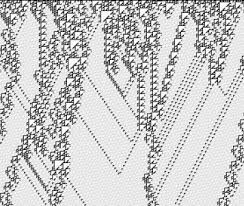
\includegraphics{rule110.jpeg}
\caption{Excerpt from the state sequence produced by Wolfram's \textit{Rule 110}
one-dimensional cellular automaton}
\end{marginfigure}

Wolfram and others have suggested that some natural processes that were
previously thought to evolve by natural selection are instead
manifestations of things that nature found "easy" to accomplish using
the same fundamental principles that underlie simple automata.

In this work, we analyze simple, rule-based graph automata using simulations of abstract
machines. Our machines operate on the same principles as
cellular automata but use a graph, rather than a "tape" or grid, as a substrate.
Where cellular machines define cell adjacency spatially, our machines use graph topology.
We discuss the machines' behavior under varied rules and explore a genetic search
algorithm for finding rules that yield terminal graphs with specific characteristics.


\section{Methods}

Two similar rule-based automata, \textbf{Machine C} and \textbf{Machine CM}, were designed
and implemented in simulation. The simulators were run repeatedly, using rules
selected at random from a large universe of possibilities. Measurements were recorded as the graphs
evolved through each run. The resulting database accumulated data on many thousands of runs. The body of data
was analyzed macroscopically, using aggregate statistics, and microscopically, by inspecting
statistical and graphic snapshots from individual runs.

\begin{marginfigure}
\hspace{3em}
\includegraphics[width=2.5cm]{evol2a_0.ps}
\end{marginfigure}

\begin{marginfigure}
\hspace{3em}
\includegraphics[width=2.5cm]{evol2a_1.ps}
\end{marginfigure}

\begin{marginfigure}
\hspace{3em}
\includegraphics[width=2.5cm]{evol2a_2.ps}
\end{marginfigure}

\begin{marginfigure}
\hspace{3em}
\includegraphics[width=2.5cm]{evol2a_3.ps}
\end{marginfigure}

\begin{marginfigure}
\hspace{3em}
\includegraphics[width=2.5cm]{evol2a_4.ps}
\caption{Four iterations of machine \textbf{C}, rule 509914832650994,
beginning with a randomly generated 32-node graph and terminating in a
static configuration.}
\end{marginfigure}

Each simulation run begins with a selected rule and a randomly generated graph. It proceeds by
iteratively modifying the graph's edges and node states according to the rule.
Each rule is effectively a simple program  that specifies, based on the state
of each node and its neighbors, how local changes should be applied during an
iteration.

\subsection{Graph Composition}

Nodes may be in one of two states: \textit{black} or \textit{white}.
Graph topology is restricted in order to simplify rule design. For the
\textbf{CM} machine:

\vspace{1mm}
\begin{itemize}
\setlength{\itemindent}{2em}
    \item Edges are directed.
    \item Nodes have out-degree of exactly two.
    \item "Self-linking" edges are permitted.
\end{itemize}
\vspace{2mm}
The \textbf{C}  machine's graphs are more narrowly defined by adding the
restriction:
\begin{itemize} 
\setlength{\itemindent}{2em}
    \item Multiple, like-directed edges between two nodes are prohibited.
\end{itemize}
\vspace{2mm}

\textbf{C} and \textbf{CM} machines operate using the same rule structures.
A single rule is chosen for each run. Each execution
begins on a graph that has been randomly generated
to conform to its machine's topological restrictions. Both machines maintain conformance
throughout the run. In applying some rules, \textbf{C} creates prohibited
structures. When this occurs, a "pruning" process selectively
removes nodes and edges to restore conformance before proceeding with the
next iteration. The \textbf{CM} machine does not need this process because
it is structurally incapable of altering its graph in a way thati violates its more
relaxed structure restrictions. \textbf{CM} is otherwise identical to \textbf{C}.  

An initial, random graph of N nodes is constructed by assigning each node
a \textit{black} or \textit{white} state with equal likelihood.
Two outbound edges are attached to each node, with
the destination of each selected at random from all nodes. For \textbf{C} runs, the
generator observes the constraint that the edges cannot share the same destination node.
In all initial graphs, nodes have out-degree 2, but in-degree can vary from 0 to N.
Initial graphs are a subset of the class of Erdos-Renyi random graphs (citation needed)
\textit{G(n, p)} where \textit{n} is the number of nodes and \textit{p} is the probability
that two nodes are connected by an edge. Because all graphs have fixed out-degree 2,
the generation process creates random variation only in the nodes' in-degrees. As a result,
each initial graph is a member of \textit{G(n, p)} where \textit{p} is a function
of graph size \textit{n} (approximately \( 4 / (n - 1) \)).

\subsection{Rule Structure and Application}

At the start of each simulation run, a rule is selected and an initial graph
is generated.  The simulation proceeds in a series of
iterations. During each, the rule is applied at each node, yielding a draft
version of a new graph. For machine \textbf{CM}, the draft immediately becomes
the input for the next iteration. In \textbf{C}, the draft may require pruning
before becoming input to the next iteration. 

During an iteration, each node in the current graph is examined in turn.
The combined \textit{black}/\textit{white} states of the node and its two neighbors\footnote{
\textit{Black} is interpreted as zero, \textit{white} as one. In
all cases, "neighbor" is used to indicate a node at the destination end of one of a node's out-edges.}
are used to select one of the rule's eight constituent parts; the selected part, in turn,
controls the changes that are made to the node's state and its out-edges in
the developing draft copy. Rules encode change instructions as follows:

A rule comprises eight parts, each corresponding to one of the possible compound, or "triad" states
of a node and its neighbors. Each rule-part specifies replacement values for
the node's state and the destinations of its out-edges
(it is convenient to refer to a node's two out-edges as "left" and "right").
The replacement node state is either \textit{black} (\textit{B}) or \textit{white} (\textit{W}).
The replacement edge destinations (Figure \ref{fig:Sixlabeled}) are each one of:

\vspace{1mm}
\begin{itemize}
\setlength{\itemindent}{2em}
    \item \textit{L} - the node's current left-edge destination
    \item \textit{R} - the node's current right-edge destination
    \item \textit{LL} - the current destination of its left neighbor's left-edge
    \item \textit{LR} - the current destination of its left neighbor's right-edge
    \item \textit{RL} - the current destination of its right neighbor's left-edge
    \item \textit{RR} - the current destination of its right neighbor's right-edge
\end{itemize}
\vspace{2mm}
A rule might be represented symbolically as a set of triples
(\textit{<new left-edge destination>},
\textit{<new right-edge destination>},
\textit{<new node state>}), for example:
\[
\aunderbrace[l1r]{(L,L,B)}_{0}\aunderbrace[l1r]{(R,RR,W)}_{1}\aunderbrace[l1r]{(L,R,W)}_{2}\aunderbrace[l1r]{(LL,R,B)}_{3}\aunderbrace[l1r]{(L,LL,B)}_{4}\aunderbrace[l1r]{(RL,RR,W)}_{5}\aunderbrace[l1r]{(RR,RR,B)}_{6}\aunderbrace[l1r]{(R,L,B)}_{7}
\]
in which each triple is a rule-part to be applied at nodes having a
triad state equal to the part's index position in the rule string. For coding purposes, rule
numbers are carried as mixed-radix integers between 0 and
$(6 \times 6 \times 2)^8 = 722,204,136,308,736$.

\begin{marginfigure}
\vspace{-5mm}
\hspace{-2em}
\includegraphics[height=3cm]{sixlabeled.ps}
\caption{The six possible new destinations for node \textbf{*}'s out-edges}
\label{fig:Sixlabeled}
\end{marginfigure}

\vspace{1mm}
After all nodes in the original graph have been processed,
the resulting draft copy is pruned if necessary.
Applicable only for machine \textbf{C}, the pruning step removes
any like-directed edges (multi-edges) that have been created between pairs
of nodes in the draft copy; the process, described in more detail below,
selectively removes nodes and redirects edges, cascading as required,
until no prohibited structures remain.
If it is not empty, the pruned graph becomes the starting point for the next iteration;
if it is empty, it is said to have collapsed.
A simulation run ends when (1) the graph collapses, (2) a state cycle is detected,
or (3) a maximum number of iterations is reached.

\subsection{The \textbf{C*} Machines' Random Counterparts, \textbf{R} and \textbf{RM}}

To help gauge the extent to which machines \textbf{C} and \textbf{CM}
introduce order as they transform random starting graphs, simulators for counterpart
machines \textbf{R} and \textbf{RM} were constructed. Like the rule-based \textbf{C} and
\textbf{CM} (\textbf{C*}) machines, these change the graph iteratively, but make their
changes \textit{randomly}.
As with the \textbf{C*} machines, though, the scope of edge destination changes for each node is
limited to nodes reachable in its "two-hop" neighborhood. (The random machines need not alter nodes' states
because node states have no effect on the \textbf{R*} machines' actions).
The \textbf{R} machine applies the same pruning process that \textbf{C} uses. As
with \textbf{CM}, no pruning step is required in \textbf{RM} simulations because
no prohibited structures can be generated by the \textbf{*M} machines.

\begin{table}
\caption{Machine Characteristics}
\centering
\begin{tabular}{lccc}
\toprule
Machine & New Edge Selection & Multi-edges & Pruning Performed \\
\midrule
\textbf{C} & \textit{Rule-based} & \textit{No} & \textit{Yes} \\
\textbf{R} & \textit{Locally Random} & \textit{No} & \textit{Yes} \\
\cmidrule(r){2-4}
\textbf{CM} & \textit{Rule-based} & \textit{Yes} & \textit{No} \\
\textbf{RM} & \textit{Locally Random} & \textit{Yes} & \textit{No} \\
\bottomrule
\end{tabular}
\label{tab:Tab1}
\end{table}
\vspace{3mm}

\subsection{Graph Pruning}

Changes to out-edge destinations, whether made randomly by machine \textbf{R}, or based on \textbf{C}'s
rules, can introduce multi-edges. These prohibited structures
arise as the machine's iteration logic creates a first-pass, "draft" copy of the transformed graph.
the draft copy is pruned to restore conformance with structure restrictions before
the following iteration begins.
The diagram in Figure \ref{fig:Pruning} shows the two kinds of prohibited structures
that can occur and illustrates the restorative changes made in the pruning step.

\begin{figure}
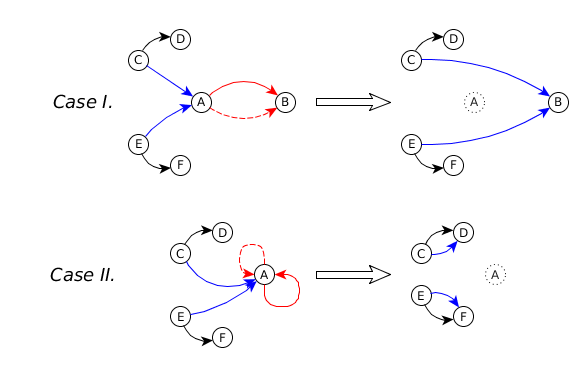
\includegraphics{pruning.png}
\caption{\textbf{Pruning.} Resolution methods for two variations of a (red) prohibited structure.
In both cases, edges originating at node A are eliminated; edges in blue are redirected.
Case II creates two case I-type structures that require further resolution.}
\label{fig:Pruning}
\end{figure}

Both types of changes eliminate the node at which the offending edge pair
originates (labeled "A" in the illustrations), along with the edge pair.
In case I, all edges inbound to the eliminated node are redirected to 
the destination (shown as node "B") of its to-be-eliminated edge pair.
Redirected edges are shown in blue.

Lacking such a natural new destination for the inbound edges in case II, the
pruning process instead moves the problem "upstream"---any edge inbound to
the eliminated node is redirected to the same destination node as that of
its origin node's other out-edge. This, of course, immediately creates
case I structure violations for all such origin nodes; these violations must also be
resolved before the next iteration can begin.
Case II resolutions \textit{always} create additional structure violations;
case I resolutions may or may not. In either case, cascades can result. These
cascades, and the resulting reductions in graph size, are common in both
\textbf{C} and \textbf{R} simulations.

\subsection{The Automaton Simulator(\textit{Explorer})}

Input parameters and statistics gathered. Data base and analysis tooling.
Constituent packages. How parameter values were selected and varied.


\subsection{The Rule-space Searcher (\textit{Searcher}")}

The rule-space for machine \textbf{C} is vast and incoherent. It comprises
$7.2 \times 10^{14}$ rules; numerically similar rules produce
very dissimilar behaviors and yield widely varying terminal graph states.
We developed a genetic search algorithm for finding rules the produce terminal
graph states with specific characteristics such as high clustering coefficients, or
a large number of (separate) connected components. A "fitness" function
quantifies the relative extent to which a rule produces a terminal graph
with the desired characteristics.

The search proceeds by first creating a pool of randomly selected rules, then
improving aggregate fitness by iteratively replacing lower-fitness rules
with new ones. The replacement rules are synthesized by
choosing two existing rules with relatively high fitness and "crossing" them,
possibly mutating one of them before crossing. The process iterates, terminating
either when the pool reaches a target fitness or when an iteration limit
is reached. Successful searches terminate with a pool having significantly
higher fitness than that of randomly generated pools.

A rule is mutated by replacing one or more of its components with a new,
randomly chosen value. Two rules are crossed by randomly choosing one or
more of their components and exchanging them. The likelihood of a mutation
occurring is controlled by the \textit{probMutation} parameter.

The search proceeds in generations. Each successive generation creates a new
pool of rules from the previous generation's by repeatedly choosing pairs
of rules from the previous pool, mutating and crossing them, then adding
the chosen rules and their new offspring to the new pool until
it is full. The process repeats until \textit{maxGenerations} have been
generated.

Rules with relatively high fitness are selected from a pool using
a list of rules in order of decreasing fitness. Each entry
is accompanied by cumulative fitness, summed from the beginning
of the list. A choice is made by choosing a target fitness value
randomly

%------------------------------------------------

\section{Results}

Our first task was to understand the characteristic behaviors of each
machine, comparing the machines and their random counterparts.
In this section, a survey of qualitative and quantitative simulation results is
presented, followed by an examination of more specific aspects of behavior.

\subsection{Summary of End States---Cycles and Collapses}

Each simulation run begins with a finite graph, and each iteration
either maintains the number of nodes or, in the cases of \textbf{C} and \textbf{R},
reduces it by pruning.  It is consequently certain that the machines always terminate,
either in a state cycle or in a graph collapse; this holds true
for all types: \textbf{C}, \textbf{CM}, and their random counterparts \textbf{R} and \textbf{RM}.
The possibility that a graph will traverse an astronomical number
of states\footnote{The number of possible states for an N-node graph with
out-degree restricted to 2 is:
\[
2^N\cdot\binom{N}{2}^N
\]
}
before revisiting a previous one, however, limits the simulator's ability to
detect cycles. If the simulator reaches a maximum number of iterations
before its machine terminates, the simulation outcome is recorded as "undetermined."
A summary of outcomes for all runs is given in Table \ref{tab:Tab2}.

\begin{table}
\caption{Simulation Outcomes, All Runs}
\centering
\begin{tabular}{lrcr}
\toprule
Machine & Cycling & Collapsed & Undet. \\
\midrule
\textbf{C} & 40.77\% & 59.22\% & 0.01\% \\
\textbf{R} & 0\% & 100\% & 0\% \\
\cmidrule(r){2-4}
\textbf{CM} & 99.07\% & --- & 0.03\% \\
\textbf{RM} & 100.00\% & --- & 0\% \\
\bottomrule
\end{tabular}
\label{tab:Tab2}
\end{table}
\vspace{3mm}

The reason that nearly all \textbf{CM} runs end in state cycles is
intuitive---because \textbf{CM} allows multi-edges, it tends to generate structures
like those in Figure \ref{fig:Multiedges} regardless of which rule is governing its execution.
As these structures enter the graph, they 
shrink the number of possible new out-edge destinations for their origin nodes,
progressively decreasing the number of possible new states in the graph overall.

Less inutuitive is the finding that all \textbf{RM} runs end in cycles---it would
seem that this machine's continuously random edge reassignments would
make state cycles impossible. In fact, \textbf{RM}'s graphs invariably devolve
to configurations in which every node's six possible "new" out-edge destinations
are, in fact, all the same node---the previous destination node of both its
out-edges---resulting in no change to the edges and causing a tight, one-state cycle.
An example of such a graph appears in Figure \ref{fig:TerminalRMGraph}.

%\begin{marginfigure}
%\hspace{1em}
%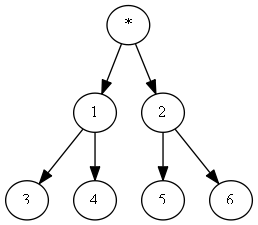
\includegraphics[height=3cm]{sixchoices.png}
%\caption{For each edge originating at the "*" node, there are six possible new destinations. (These
%are not necessarily six different nodes, but are more likely to be distinct nodes when
%multi-edges are not present.)}
%\label{fig:Sixnumbered}
%\end{marginfigure}

\begin{marginfigure}
\includegraphics{multiedges.ps}
\caption{Structures with multi-edges reduce the number of possible new edge destinations for
the origin ("*") node during each machine iteration.}
\label{fig:Multiedges}
\end{marginfigure}

\begin{marginfigure}
\includegraphics{terminal_RM_graph.ps}
\caption{A representative terminal graph from an \textbf{RM} simulation. The
configuration is a one-state cycle even under locally random edge reassignment.}
\label{fig:TerminalRMGraph}
\end{marginfigure}

The prohibition of multi-edges in machines \textbf{C} and \textbf{R}
necessitates the removal of prohibited structures when they arise. The
number of nodes in the graph can consequently decrease during execution,
often to the point of complete collapse.
Machine \textbf{R} is far more likely to produce graph collapses than
\textbf{C} is (99.9\% vs. 59.2\% of runs). The reason is similar to the reason
that \textbf{*M} machine runs cycle: \textbf{R} and \textbf{RM} share the same
random edge rerouting logic, and produce multi-edges with equal likelihood. These are allowed to
remain in \textbf{RM}'s graph, but must be pruned out of \textbf{R}'s graph
before it can continue with execution, reducing its node count and making collapse
more likely. The number of multi-edges \textbf{C} produces, on the other hand,
is determined by the rule under which it runs, and consequently varies widely as
the machine is run with different rules.

\clearpage

\begin{table}
\centering
\caption{Comparison of Graph Measures, \textbf{C} vs. \textbf{R}}
\begin{tabular}{ll}\toprule
\addlinespace[3mm]
Statistic  & Comparison \\ \midrule
\addlinespace[2mm]

\makecell[tl]{
Average \\%
Run Length \\%
\& Terminal \\%
Graph Size} &
\makecell[tl]{
Between \textbf{C} and \textbf{R} runs ending in collapse, \\%
\textbf{C} runs average nearly twice the number of \\%
iterations (Figure \ref{fig:OutcomesNriterAvg}) and end with much higher \\%
pre-collapse node counts (Figure \ref{fig:OutcomesFinnnDist}). They \\%
run longer and their node counts \\%
"fall farther" when they collapse. \\%
\\%
\textbf{C} runs that end in state cycles terminate \\%
with higher average node counts than \\%
those for collapsing runs, despite \\%
averaging more than twice the run length. \\%
\\%
Machine \textbf{C} runs lengths correlate \\%
with terminal graphs sizes except in \\%
the case of the largest sizes, which tend \\%
to be produced in somewhat shorter runs. \\%
run lengths decrease somewhat (Figure \ref{fig:NriterXFinnn})} \\

\vspace{2mm}
\makecell[tl]{
Average \\%
Clustering \\%
Coefficient} &
\makecell[tl]{
Terminal clustering coefficients for \\%
machine \textbf{C} are smaller than \\%
those for \textbf{R} in the large majority \\%
of cases (Figure \ref{fig:OutcomesAccDist}).} \\

\vspace{2mm}
LastTopic & \\ \bottomrule
\end{tabular}
\label{tab:TabQ}
\end{table}

\begin{marginfigure}
  \vspace{-8cm}
  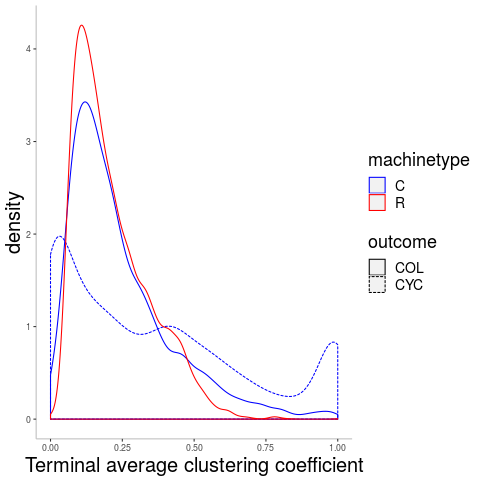
\includegraphics{outcomes-acc-dist.png} \\
  \caption{Distribution of terminal average clustering coefficients for machine \textbf{C} (cycling), \textbf{C} (collapsing), and \textbf{R} (collapsing).}\label{fig:OutcomesAccDist}
\end{marginfigure}

\begin{figure}[!h]
   \begin{floatrow}
\ffigbox{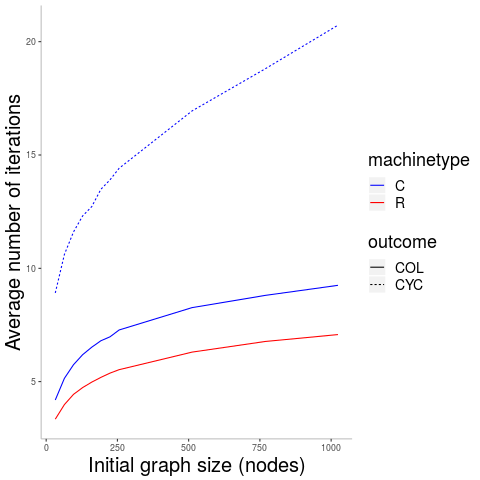
\includegraphics[width=\linewidth]{outcomes-nriter-avg.png}}%
    {\caption{Average number of iterations for machine \textbf{C} (cycling), \textbf{C} (collapsing), and \textbf{R} (collapsing).}\label{fig:OutcomesNriterAvg}}
\hfill
\ffigbox{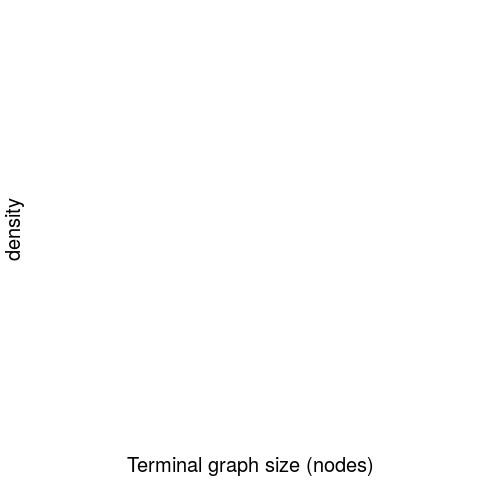
\includegraphics[width=\linewidth]{outcomes-finnn-dist.png}}%
    {\caption{Distribution of terminal graph sizes for machine \textbf{C} (cycling), \textbf{C} (collapsing), and \textbf{R} (collapsing) with initial graph size 1031.}\label{fig:OutcomesFinnnDist}}
    \end{floatrow}
\end{figure}

\clearpage

\subsection{In-Degree Entropy}

Machine \textbf{C}, on average, generates graphs with a larger 
maximum in-degree than in the random case of machine \textbf{R}, and also produces a
larger number of distinct in-degrees.

Shannon's entropy [citation needed], computed on summary in-degree statistics and
normalized,\footnote{
Normalized entropy calculation: \\
\vspace{2mm}
$p_{k}=$ fraction of nodes with degree k \\
$K=$ number of distinct in-degrees \\
\vspace{2mm}
$entropy = \frac{\sum_{k=1}^{K} p_{k} log_{2}p_{k}} {log_{2}K}$}
can be regarded a measure of a graph's "randomness."
As would be expected, entropy is consistently large in the randomly generated
initial graphs. Between the \textbf{R} and \textbf{C} machines, entropy in the terminal
graphs for \textbf{C} is lower than that for the randomly operating R (Figure \ref{fig:figE}).

The drop in average entropy between initial graphs and the \textbf{R} machine's terminal
graphs seems surprising on its face, but is accounted for by the restriction that
\textbf{R}'s topological changes, like \textbf{C}'s, may only redirect a node's out-edge
within its two-hop neighborhood.
The effect is to "localize" the randomness, abruptly increasing apparent order in the
random graph as soon as the first iteration is finished.

\begin{marginfigure}
  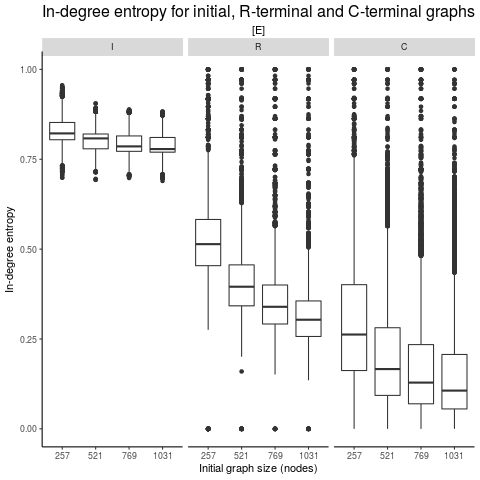
\includegraphics{figE.png}
  \caption{In-degree entropy is largest in initial random graphs,
        smaller for \textbf{R}'s terminal graphs, and smallest for \textbf{C}'s terminal graphs.}
  \label{fig:figE}
\end{marginfigure}

\subsection{Sensitivity to Initial Conditions}

\subsection{Degree Distribution}

This is where things get more interesting.

For this one, we'll have to dust off the old self-organizing criticality
references. Are collapses like sandpile avalanches?

\subsection{Designed Rules}
%Made to Order?
%Learning the Hard Way?
%Designer Rules? Rules by Design?

\subsection{Interesting Configurations}
%Photo Opps?
Sorter?

%------------------------------------------------

\section{Discussion}

Possible areas for further investigation:

\begin{itemize}
    \item Search strategies for rules with specific characteristics.
    \item Encodings of more complex graph structures.
    \item Exploring mathematical parallels.
    \item Investigating variations on the machines, both simpler and more complex.
\end{itemize}

A statement requiring citation \cite{Figueredo:2009dg}.

%----------------------------------------------------------------------------------------
%	REFERENCE LIST
%----------------------------------------------------------------------------------------

\begin{thebibliography}{99} % Bibliography - this is intentionally simple in this template

\bibitem[Figueredo and Wolf, 2009]{Figueredo:2009dg}
Figueredo, A.~J. and Wolf, P. S.~A. (2009).
\newblock Assortative pairing and life history strategy - a cross-cultural
  study.
\newblock {\em Human Nature}, 20:317--330.
 
\end{thebibliography}

\vspace{1cm}

\emph{This handout was based on an article I originally wrote for the Carolinia Farm Stewardship newsletter, March-April 2004.}

\end{document}
